\documentclass[12pt,a4paper]{article}
\usepackage[T1]{fontenc}
\usepackage[utf8]{inputenc}
\usepackage{microtype}
\usepackage{mathptmx}
\usepackage{amsmath}
\usepackage[margin=2.5cm]{geometry}
\usepackage{setspace}
\usepackage{authblk}
\sloppy
\onehalfspacing
\usepackage{graphicx}
\usepackage{booktabs}
\usepackage[colorlinks=true,linkcolor=blue,citecolor=blue,urlcolor=blue]{hyperref}
\usepackage[superscript,biblabel]{cite}
\usepackage{enumitem}

\title{\bfseries Identification of Long Non-Coding RNA Signatures for Diagnosis and Prognosis of Colorectal Cancer via Machine Learning}

\author[1,$\dagger$]{Zhuha Zhou}
\author[1,$\dagger$]{Yongyu Bai}
\author[2]{Qigang Xue}
\author[3]{Zhuxian Zhou}
\author[1,*]{Shaoliang Han}

\affil[1]{Department of Gastroenterology Surgery, The First Affiliated Hospital of Wenzhou Medical University, Nanbaixiang Street, Ouhai District, 325000, Wenzhou, Zhejiang, China}
\affil[2]{Department of Hepatobiliary and Pancreatic Surgery, The First Affiliated Hospital of Wenzhou Medical University, Nanbaixiang Street, Ouhai District, 325000, Wenzhou, Zhejiang, China}
\affil[3]{Center for Bionanoengineering, College of Chemical and Biological Engineering, Zhejiang University, Hangzhou 310027, China}

\date{}

\newcommand{\daggernote}{$^\dagger$These authors contributed equally to this work.}
\newcommand{\starnote}{$^*$Correspondence: ShaoliangHan@wmu.edu.cn}

\date{}

\begin{document}
\maketitle

\vspace{-12pt}
\begin{center}\small\daggernote\qquad\starnote\end{center}

\begin{abstract}
\noindent
\textbf{Background:} Colorectal cancer (CRC) remains a leading cause of cancer-related mortality, yet clinically actionable molecular biomarkers for early detection and prognosis are still limited. Long non-coding RNAs (lncRNAs) have emerged as promising biomarkers, but identifying robust signatures from high-dimensional transcriptomic data requires systematic computational strategies.

\textbf{Methods:} We integrated differential expression analysis with elastic-net regularized Cox regression and five machine learning classifiers to discover lncRNA signatures with both diagnostic and prognostic value in CRC. Using the TOIL-recomputed TCGA--GTEx dataset (349 non-tumor, 290 tumor samples) and TCGA-COAD clinical follow-up data (428 patients), we identified 17 candidate lncRNAs and further refined them to an 8-lncRNA panel via stepwise multivariate Cox regression. Prognostic performance was evaluated using Cox proportional hazards and random survival forest models; diagnostic performance was assessed using logistic regression, elastic-net logistic regression, support vector machine (SVM), random forest, and neural network classifiers.

\textbf{Results:} A Cox proportional hazards model incorporating eight lncRNAs and pathological stage stratified patients into distinct risk groups (log-rank $p < 0.0001$ in training; $p = 0.0028$ in testing), with time-dependent AUC converging to 0.725 at 8 years. Among classification models, SVM, random forest, and neural network achieved testing-set accuracies of 91.6\%, 92.2\%, and 90.6\%, respectively, substantially outperforming logistic regression (72.8\%) and elastic-net logistic regression (73.3\%).

\textbf{Conclusions:} Machine learning-driven analysis of lncRNA expression profiles can yield clinically relevant diagnostic and prognostic biomarkers for CRC. Our fully reproducible computational pipeline provides a resource for future biomarker discovery studies and independent validation.

\textbf{Keywords:} colorectal cancer, long non-coding RNA, machine learning, biomarker, diagnosis, prognosis, Cox proportional hazards, elastic net
\end{abstract}

\newpage

\section{Introduction}

Colorectal cancer (CRC) is the third most frequently diagnosed malignancy and the second leading cause of cancer-associated death worldwide, accounting for approximately 1.9 million new cases and 900,000 deaths annually~\cite{ref1}. Despite advances in screening and treatment, the majority of CRC cases are diagnosed at advanced stages, when lymph node involvement or distant metastasis has already occurred. The 5-year survival rates decline sharply from 91.1\% for localized disease to 69.8\% for regional spread and 11\% for distant metastasis, highlighting the urgent need for molecular biomarkers that enable early detection and accurate prognosis~\cite{ref1}. Alarmingly, CRC incidence among adults under 50 years has been rising since the mid-1990s in many high-income countries, underscoring the importance of developing novel diagnostic and prognostic tools.

Long non-coding RNAs (lncRNAs) are transcripts longer than 200 nucleotides that do not encode proteins but function as versatile regulators of gene expression at the epigenetic, transcriptional, and post-transcriptional levels. Accumulating evidence has demonstrated that lncRNAs participate in cancer hallmarks including proliferation, invasion, metastasis, and drug resistance~\cite{ref2}, and several lncRNAs have been specifically implicated in CRC pathogenesis through diverse mechanisms~\cite{ref3,ref4,ref5}. Because lncRNAs exhibit tissue-specific and disease-specific expression patterns, they are increasingly recognized as promising biomarkers and therapeutic targets~\cite{ref6,ref7,ref8}. However, traditional experimental approaches for discovering disease-associated lncRNAs are time-consuming and low-throughput, creating a strong incentive for computational methods that can prioritize candidates from large-scale sequencing data.

The public availability of RNA-sequencing datasets from The Cancer Genome Atlas (TCGA)~\cite{ref9} and the Genotype-Tissue Expression (GTEx)~\cite{ref10} projects has created unprecedented opportunities for transcriptome-wide biomarker discovery. Notably, the TOIL project developed by the University of California, Santa Cruz, has recomputed TCGA and GTEx raw expression data through a unified pipeline, minimizing batch effects and enabling direct comparison between tumor and normal tissues~\cite{ref11}. This harmonized resource provides a statistically well-powered foundation for identifying differentially expressed lncRNAs that distinguish CRC from normal tissue, particularly because the original TCGA-COAD cohort contains only 41 adjacent non-tumor samples, which is insufficient for robust differential expression analysis.

Machine learning has emerged as a transformative tool in CRC research, with applications spanning colonoscopy screening, histopathological diagnosis, radiomics-based prognostication, and genomic biomarker discovery~\cite{ref12}. Supervised classification algorithms can distinguish cancerous from normal tissues with high accuracy, while survival models estimate patient risk over time~\cite{ref13,ref14}. Despite these advances, the application of machine learning to lncRNA-based biomarker discovery remains relatively underexplored. The \texttt{caret} package in R provides a unified interface that streamlines model training, hyperparameter tuning, and performance evaluation across diverse algorithms~\cite{ref15}. Zhang \textit{et al.} developed CRlncRC, a machine learning-based classifier for cancer-related lncRNAs that integrates multiple optimization strategies~\cite{ref16}. However, studies that simultaneously assess diagnostic and prognostic utility of lncRNA signatures using standardized, reproducible machine learning pipelines remain scarce~\cite{ref17}. Although machine learning holds tremendous promise for medical applications, translating computational models into clinically actionable tools requires rigorous validation and attention to interpretability~\cite{ref18}.

In this study, we designed an integrated computational pipeline to identify lncRNA signatures with dual diagnostic and prognostic value in CRC. Our pipeline combines differential expression analysis across the harmonized TCGA--GTEx dataset, elastic-net regularized Cox regression for feature selection, multivariate Cox proportional hazards modeling and a random survival forest for prognostic evaluation, and five classification algorithms for diagnostic prediction. The identified lncRNA panel yielded excellent discriminative performance in distinguishing tumor from normal tissue and provided stable, time-dependent prognostic stratification beyond routine pathological staging.

\section{Materials and Methods}

\subsection{Data Acquisition and Preprocessing}

We obtained gene expression data from two complementary sources. The harmonized TCGA--GTEx dataset (TOIL recomputed, $\log_2(\text{FPKM}+0.001)$ normalized) was downloaded from the UCSC Xena platform (\url{https://toil.xenahubs.net}). The TCGA-COAD gene expression data (HTSeq-FPKM) and corresponding clinical follow-up information were retrieved from the NCI Genomic Data Commons (\url{https://portal.gdc.cancer.gov}) via the FirebrowseR R package~\cite{ref19}. Genes were mapped to GENCODE v22 (TCGA-COAD) and v23 (TCGA--GTEx) annotations, respectively.

For the TCGA--GTEx dataset, colon samples were extracted by filtering phenotype annotations for site = ``Colon,'' yielding 349 non-tumor samples (GTEx colon + TCGA solid tissue normal) and 290 tumor samples (TCGA-COAD primary tumor). Genes with expression values below 0.1 in more than 60\% of samples were removed as uninformative. For the TCGA-COAD dataset, technical replicate samples (22 cases) were condensed by averaging, and genes with expression below 0.5 in more than 60\% of samples were removed. Expression values were $\log_2(\text{FPKM}+1)$ transformed. Clinical follow-up data were merged with expression data, yielding 428 patients with complete pathological stage and survival information.

\subsection{Differential Expression and Univariate Survival Analysis}

We performed differential expression analysis between tumor and non-tumor samples in the TCGA--GTEx dataset using the \texttt{limma} package with empirical Bayes moderation~\cite{ref20}. LncRNAs were extracted by intersecting the expression matrix with GENCODE v23 long non-coding RNA annotations. For each lncRNA, univariate Cox proportional hazards regression and Kaplan--Meier analysis (with patients dichotomized by median expression) were performed using overall survival (OS) as the endpoint. LncRNAs meeting the criteria of $|\log_2\text{FC}| \geq 0.5$, Benjamini--Hochberg adjusted $p < 0.05$, log-rank $p < 0.05$, and univariate Cox Wald test $p < 0.05$ were retained as candidates.

\subsection{Regularized Cox Regression and Feature Selection}

We applied elastic-net regularized Cox regression to the candidate lncRNAs using the \texttt{glmnet} package~\cite{ref21,ref22}. The elastic net penalty combines the $L_1$ (lasso) and $L_2$ (ridge) penalties via a mixing parameter $\alpha$:

\begin{equation}
L_{\text{elasticnet}}(\hat{\beta}) = \frac{\sum_{i=1}^{n}(y_i - x_i^{\prime}\hat{\beta})^2}{2n} + \lambda\left(\frac{1-\alpha}{2}\sum_{j=1}^{m}\hat{\beta}_j^2 + \alpha\sum_{j=1}^{m}|\hat{\beta}_j|\right)
\end{equation}

Tenfold cross-validation was used to optimize $\alpha$ and $\lambda$ via minimization of the partial log-likelihood deviance. LncRNAs with non-zero coefficients at the optimal $\lambda_{\min}$ were selected as candidate features.

\subsection{Multivariate Cox Model and Survival Risk Stratification}

The follow-up dataset was randomly partitioned into training (70\%) and testing (30\%) sets while preserving the distribution of survival status. Stepwise multivariate Cox regression with bidirectional selection based on AIC was applied to the training set to further refine the candidate lncRNAs. The relative risk score for each patient was computed as:

\begin{equation}
\text{RRS} = \frac{\exp\left(\sum_{i=1}^{p}\beta_i x_i\right)}{\exp\left(\sum_{i=1}^{p}\beta_i \bar{x}_i\right)}
\end{equation}

where $\beta_i$ are the fitted regression coefficients and $\bar{x}_i$ are the population average covariate values. We stratified patients into high- and low-risk groups using the median RRS as the cutoff. We used Kaplan--Meier curves and log-rank tests to compare survival between risk groups, and generated time-dependent ROC curves using the \texttt{survivalROC} R package~\cite{ref23} to evaluate the predictive performance of the RRS at multiple time points~\cite{ref24}.

\subsection{Random Survival Forest}

We constructed a random survival forest (RSF) model using the \texttt{randomForestSRC} R package~\cite{ref25} with the same covariate set (eight lncRNAs and stage), and tuned hyperparameters by grid search to minimize the OOB error: $\text{ntree} = 500$, $\text{nodesize} = \{1, \dots, 100\}$, $\text{mtry}$ initialized at $\lfloor\sqrt{p}\rfloor$. Tree splitting used the log-rank statistic, and ensemble mortality was estimated by the Kaplan--Meier estimator within each terminal node.

\subsection{Model Comparison for Survival Prediction}

We compared the discriminative performance of the Cox and RSF models using two complementary metrics. First, we computed the time-dependent Brier score via inverse probability of censoring weighting with 100 bootstrap cross-validation resamples, using the \texttt{pec} R package~\cite{ref26}. Second, we calculated the concordance index (C-index), which measures the proportion of patient pairs whose predicted and observed survival times are concordant. A Cox model using stage alone served as a reference to quantify the incremental value of the lncRNA signature.

\subsection{Classification Models for Diagnostic Prediction}

The eight lncRNAs were extracted from the TCGA--GTEx expression matrix, Box--Cox transformed to reduce skewness, and randomly partitioned into training (70\%) and testing (30\%) sets. Five classification algorithms were implemented using the \texttt{caret} R package~\cite{ref15}: logistic regression (baseline), elastic-net regularized logistic regression, random forest, SVM with radial basis function kernel, and neural network. Each model was trained with five repeats of tenfold cross-validation; hyperparameters were tuned to maximize the cross-validated AUC. Model performance was evaluated on the held-out testing set using accuracy, AUC, precision, recall, F1 score, Cohen's kappa, and cumulative gain lift curves. The \texttt{pROC} R package~\cite{ref27} was used for ROC analysis.

\subsection{Statistical Analysis}

We performed all statistical analyses using R version 3.6. We compared categorical variables using the chi-squared test (with continuity correction for $2 \times 2$ tables) and continuous variables using the $t$-test. We express results as mean $\pm$ standard deviation unless otherwise noted, and used a significance level of $\alpha = 0.05$ throughout. Model evaluation metrics were defined as:

\begin{equation}
\text{Cohen's } \kappa = \frac{p_o - p_e}{1 - p_e}
\end{equation}

\begin{align}
\text{Accuracy} &= \frac{\text{TP} + \text{TN}}{\text{TP} + \text{FP} + \text{FN} + \text{TN}}, \quad
\text{Precision} = \frac{\text{TP}}{\text{TP} + \text{FP}}, \nonumber\\
\text{Recall} &= \frac{\text{TP}}{\text{TP} + \text{FN}}, \quad
\text{F1} = 2 \times \frac{\text{Recall} \times \text{Precision}}{\text{Recall} + \text{Precision}}
\end{align}

\section{Results}

\subsection{Identification of Candidate lncRNAs Through Differential Expression and Survival Analysis}

We developed a computational pipeline to systematically identify lncRNAs with diagnostic and prognostic potential in CRC (Figure~\ref{fig1}). Starting from 58,581 genes in the TOIL-recomputed TCGA--GTEx colon dataset (349 non-tumor and 290 tumor samples), we removed lowly expressed genes (value $< 0.1$ in $> 60\%$ of samples), retaining 15,255 genes. From these, we extracted 459 lncRNAs that met at least one of our screening criteria: (i) absolute $\log_2$ fold change $> 0.5$ with Benjamini--Hochberg adjusted $p < 0.05$ in differential expression analysis, or (ii) significant association with overall survival ($p < 0.05$ in either Kaplan--Meier log-rank tests or univariate Cox regression).

We applied elastic-net regularized Cox regression with tenfold cross-validation to further select features from these 459 lncRNAs. The optimal regularization parameters were $\alpha = 0.172$ and $\log(\lambda) = -1.321$, yielding a minimum cross-validated partial log-likelihood deviance of 12.354 (Figure~\ref{fig2}). This procedure identified 17 lncRNAs with non-zero coefficients as candidate features.

The differential expression and survival analysis results for the 17 candidate lncRNAs are summarized in Table~\ref{tab1}. The majority of candidates were significantly downregulated in tumor tissue and associated with increased hazard ratios (HR). Two lncRNAs showed the opposite pattern: AC114730.3 ($\log_2$FC = 1.688, HR = 0.87) and LINC00261 ($\log_2$FC = 3.045, HR = 0.90) were upregulated in tumor tissue yet associated with decreased hazard ratios. This protective association is consistent with LINC00261's reported role as a negative regulator of cell growth that promotes differentiation and apoptosis. The expression patterns and survival associations for all 17 candidates are further detailed in Supplementary Figure~S1A.

\begin{table}[htp]
\centering
\caption{Differential expression and univariate survival analysis of the 17 candidate lncRNAs.}
\small
\begin{tabular}{lcccccc}
\toprule
\textbf{Symbol} & \textbf{Ensembl ID} & \textbf{$\log_{2}$FC} & \textbf{FDR} & \textbf{HR} & \textbf{95\% CI} & \textbf{$p$} \\
\midrule
ARRDC1-AS1 & ENSG00000203993.4 & $-$0.745 & $<0.001$ & 1.80 & (1.21--2.65) & 0.003 \\
EIF3J-AS1 & ENSG00000179523.4 & $-$0.387 & $<0.001$ & 1.70 & (1.20--2.53) & 0.004 \\
CTB-25B13.12 & ENSG00000267317.2 & 0.014 & 0.888 & 1.70 & (1.28--2.36) & $<0.001$ \\
AP006621.5 & ENSG00000255284.1 & $-$1.114 & $<0.001$ & 1.60 & (1.22--2.01) & $<0.001$ \\
RP11-644F5.11 & ENSG00000258056.2 & $-$0.327 & 0.001 & 1.60 & (1.15--2.34) & 0.007 \\
AC113189.5 & ENSG00000233223.2 & $-$0.734 & $<0.001$ & 1.50 & (1.20--1.92) & 0.001 \\
RP11-44M6.7 & ENSG00000274272.1 & $-$1.254 & $<0.001$ & 1.50 & (1.18--2.02) & 0.002 \\
LINC00174 & ENSG00000179406.6 & $-$1.016 & $<0.001$ & 1.40 & (1.11--1.72) & 0.004 \\
TNRC6C-AS1 & ENSG00000204282.4 & $-$0.140 & 0.213 & 1.40 & (1.10--1.78) & 0.006 \\
MIR210HG & ENSG00000247095.2 & 0.129 & 0.352 & 1.40 & (1.17--1.68) & $<0.001$ \\
RP11-199F11.2 & ENSG00000262251.1 & 0.244 & 0.022 & 1.40 & (1.10--1.78) & 0.006 \\
RP5-1021I20.1 & ENSG00000259065.1 & $-$1.029 & $<0.001$ & 1.30 & (1.07--1.52) & 0.007 \\
RP11-268J15.5 & ENSG00000116883.8 & $-$0.409 & 0.001 & 1.20 & (1.06--1.38) & 0.005 \\
AC156455.1 & ENSG00000256546.1 & $-$0.948 & $<0.001$ & 1.20 & (1.05--1.35) & 0.007 \\
RP11-440D17.3 & ENSG00000272913.1 & $-$0.232 & 0.152 & 1.10 & (0.91--1.19) & 0.064 \\
LINC00261 & ENSG00000259974.2 & 3.045 & $<0.001$ & 0.90 & (0.82--0.98) & 0.022 \\
AC114730.3 & ENSG00000224272.2 & 1.688 & $<0.001$ & 0.87 & (0.79--0.97) & 0.012 \\
\bottomrule
\end{tabular}
\label{tab1}
\end{table}

\begin{figure}[htp]
\centering
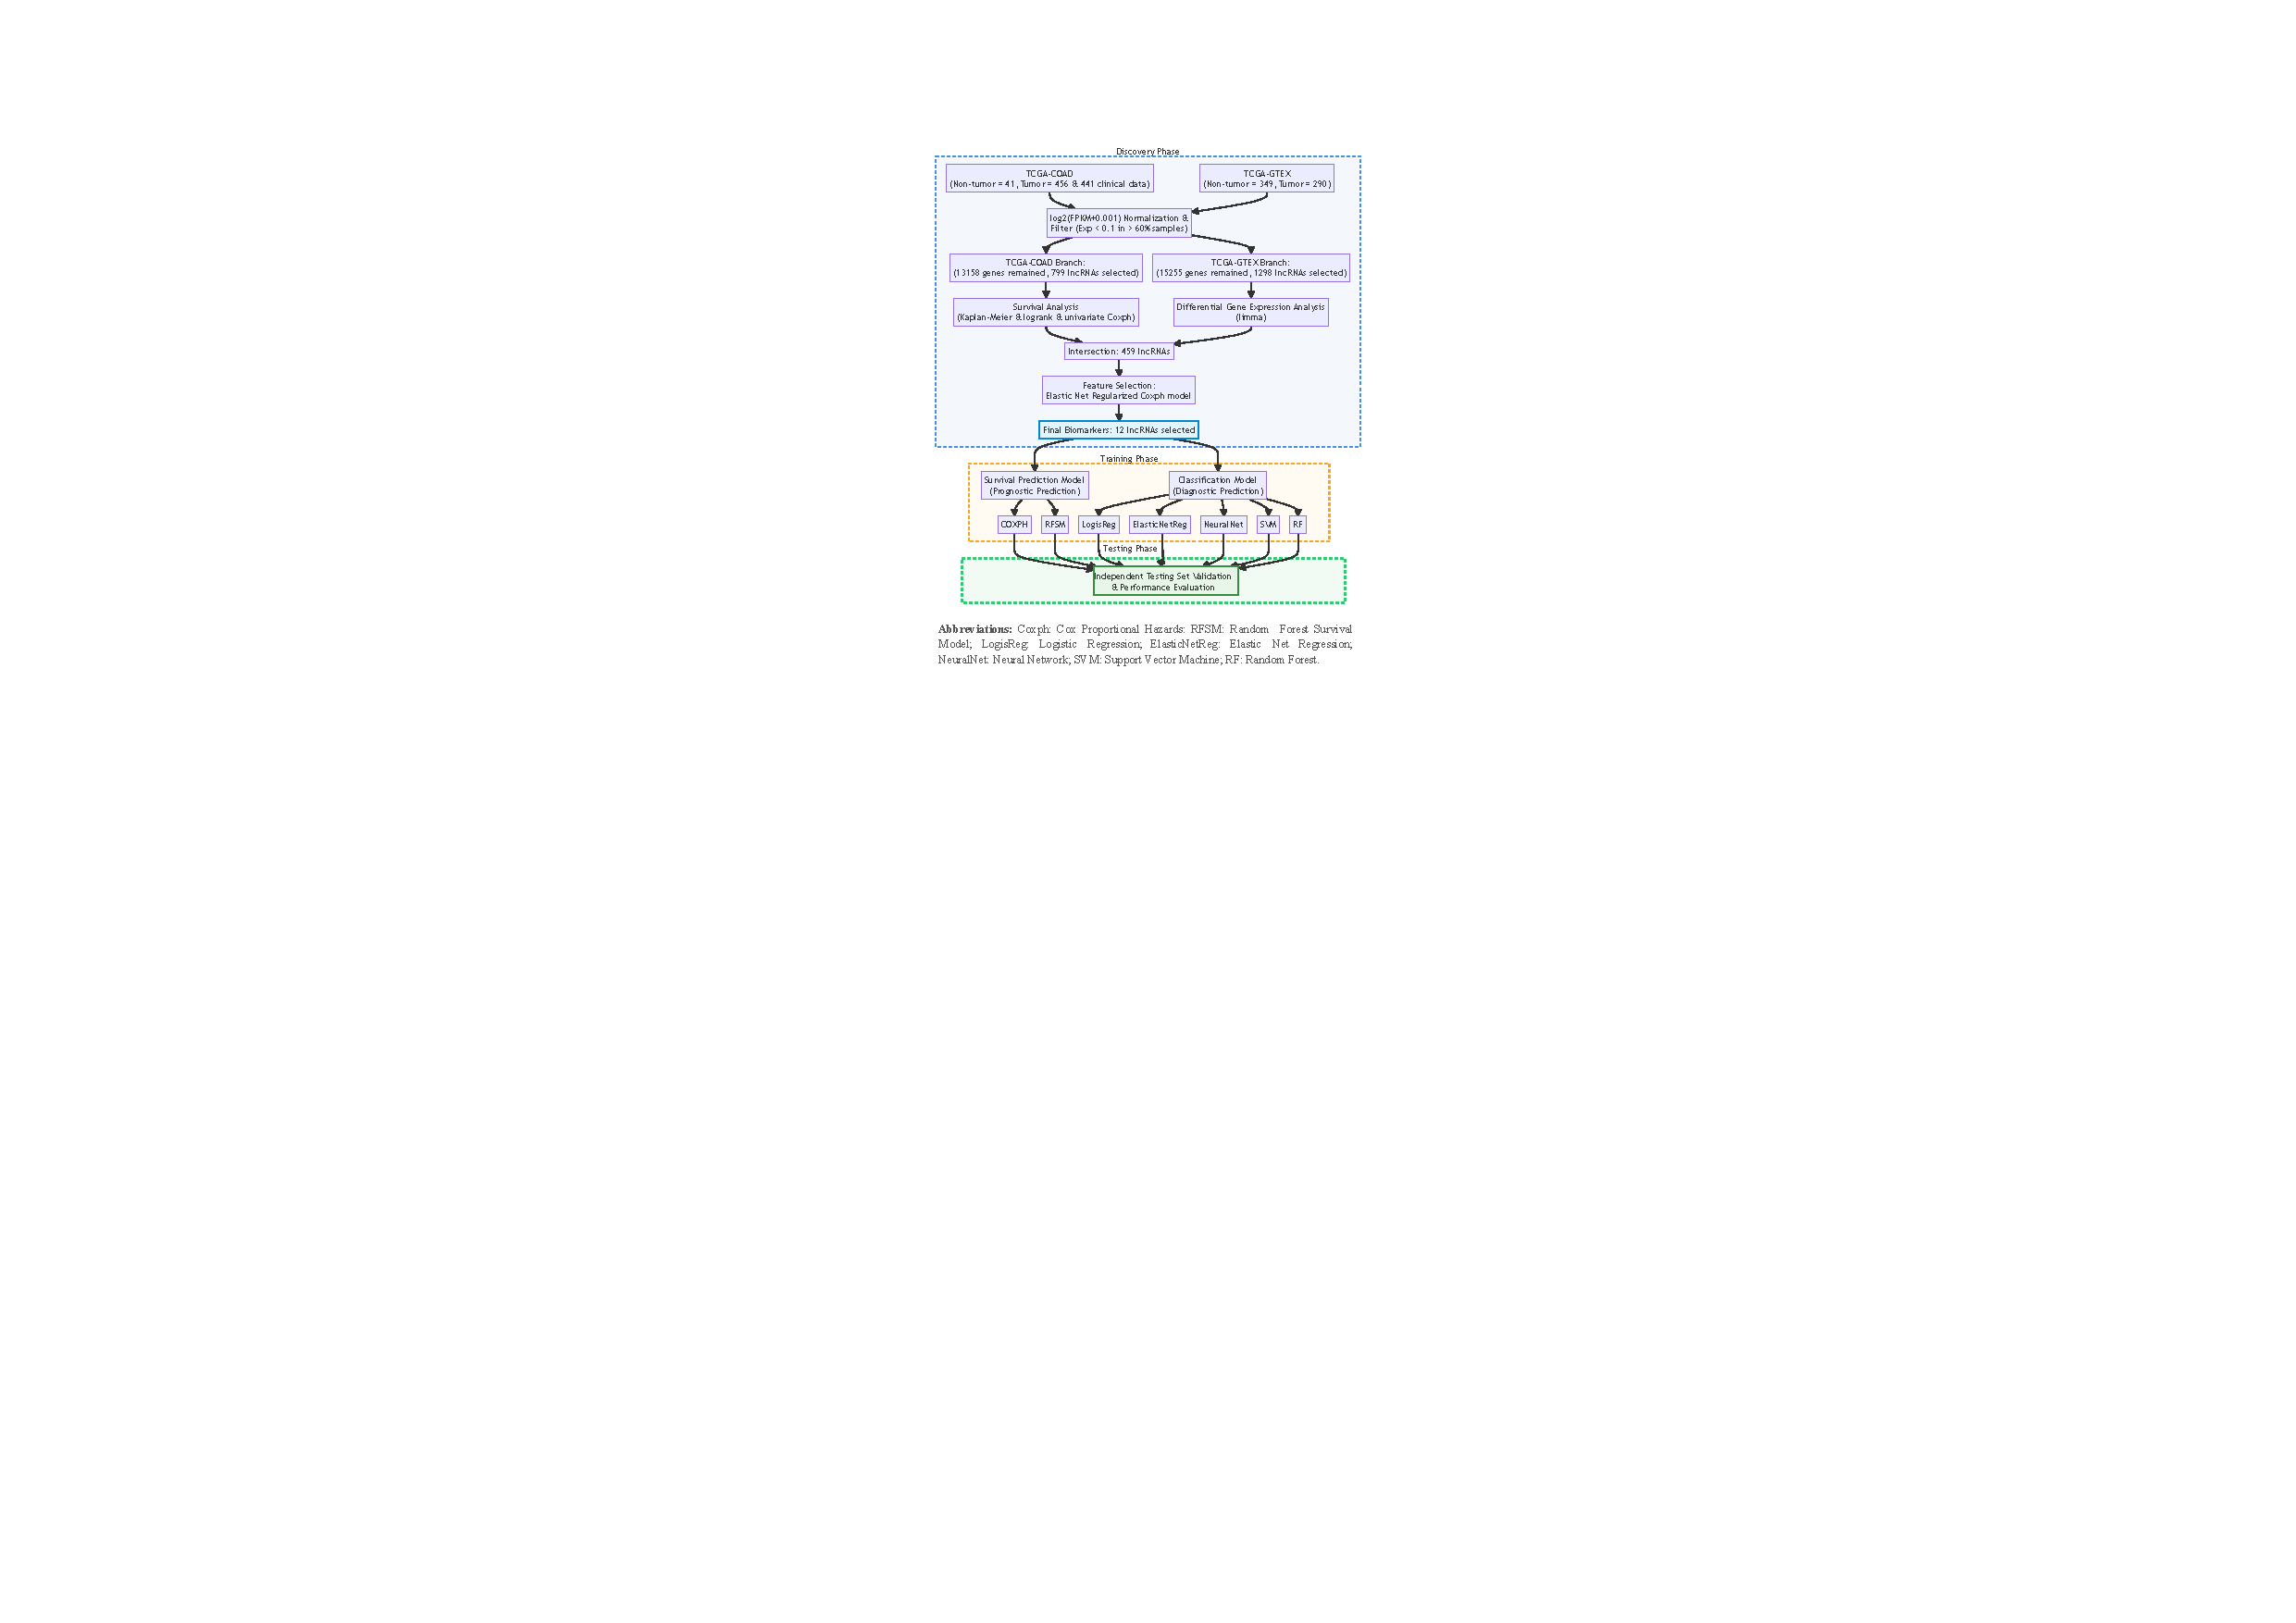
\includegraphics[width=\textwidth]{Figure-1}
\caption{Study flowchart. The TOIL-recomputed TCGA--GTEx expression data ($n = 639$ samples) were used for differential expression analysis and classification model construction. The TCGA-COAD follow-up survival data ($n = 428$ patients) were used for prognostic model development. Two survival prediction models and five classification models were constructed and evaluated.}
\label{fig1}
\end{figure}

\begin{figure}[htp]
\centering
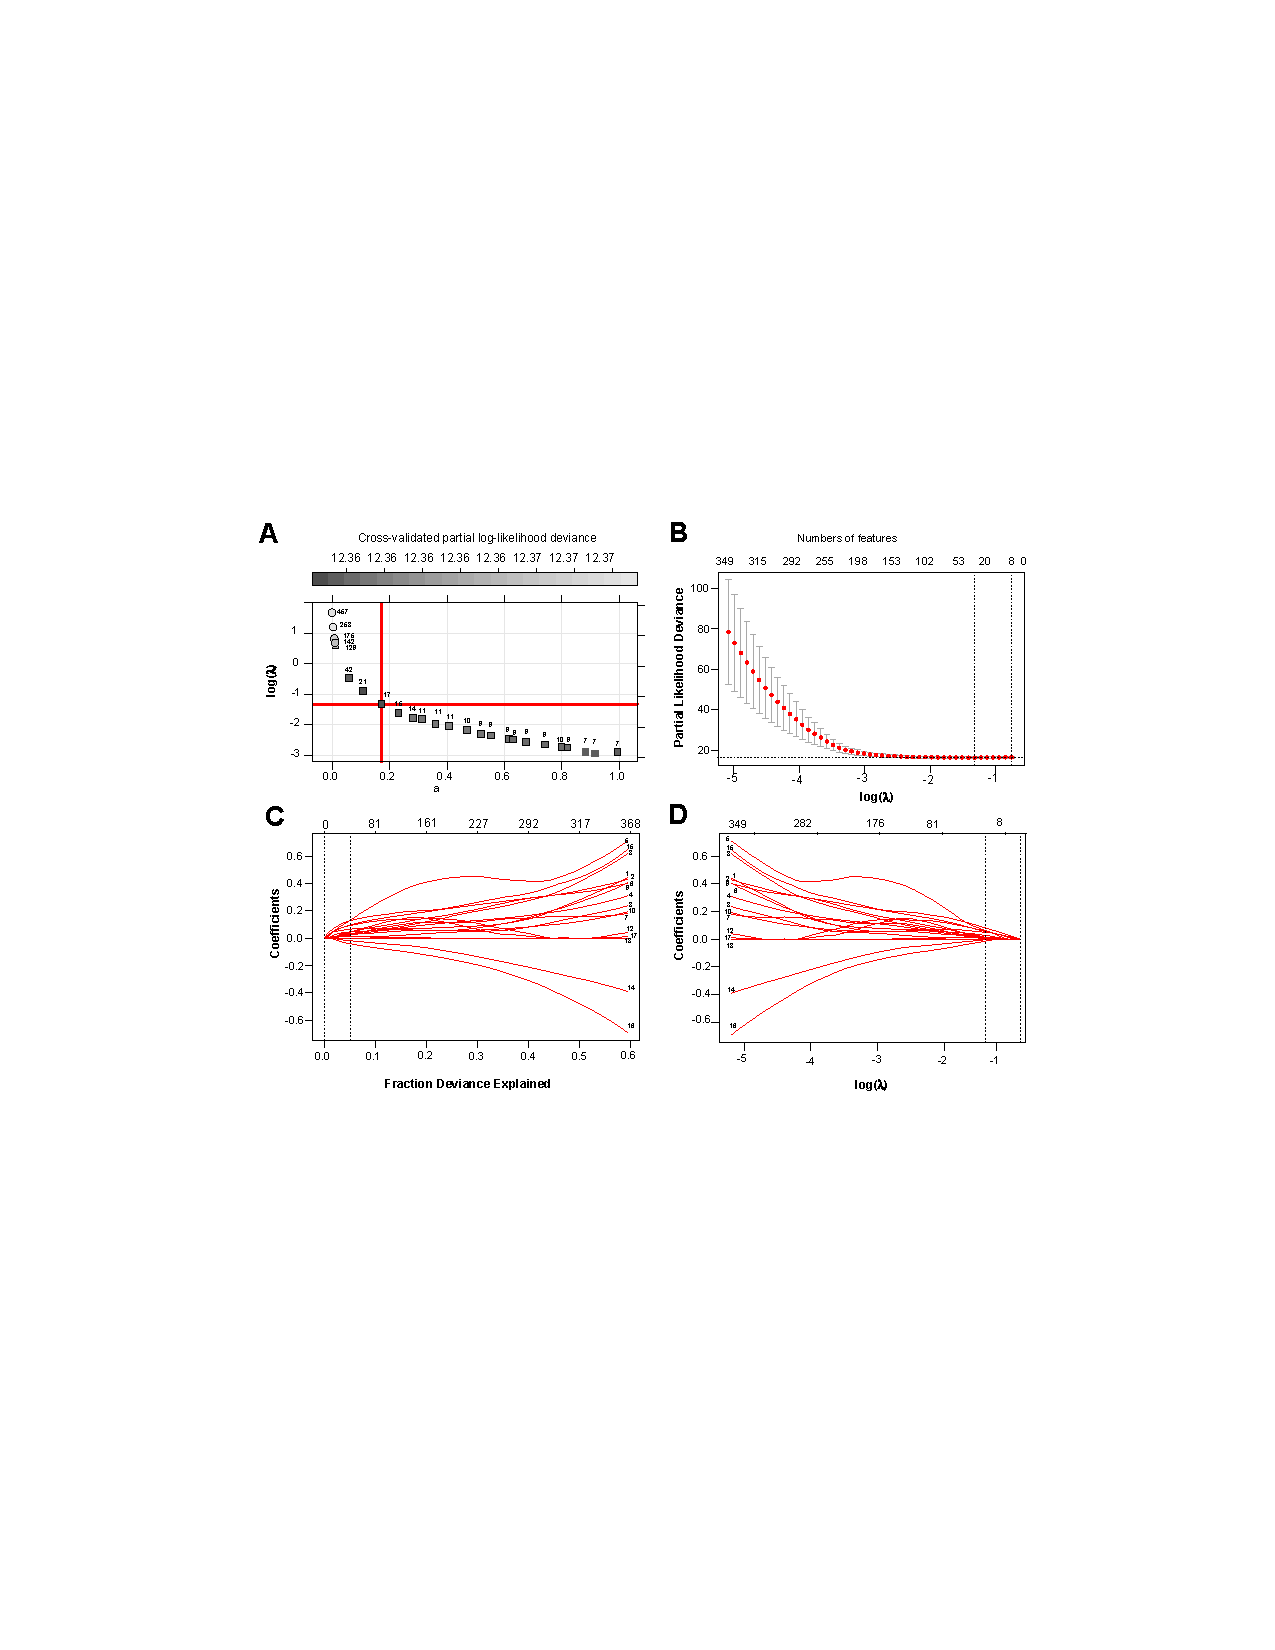
\includegraphics[width=\textwidth]{Figure-2}
\caption{Elastic-net regularized Cox regression hyperparameter tuning. \textbf{(A)} Tenfold cross-validated partial log-likelihood deviance as a function of mixing parameter $\alpha$ and $\log(\lambda)$. \textbf{(B)} Cross-validated deviance curve. \textbf{(C)} Fraction of deviance explained. \textbf{(D)} Coefficient shrinkage paths.}
\label{fig2}
\end{figure}

\subsection{Prognostic Model Construction and Survival Prediction}

We randomly partitioned the follow-up survival data into training (70\%) and testing (30\%) sets, preserving balanced distributions of survival status and clinical features (Supplementary Table~S1). Because a substantial proportion of clinical covariates contained missing values, only pathological stage---a well-established prognostic factor---was included alongside lncRNA expression in downstream models. Stage was treated as an ordinal categorical covariate with dummy coding and stage I as the reference level.

We further refined the 17 candidate lncRNAs via stepwise multivariate Cox regression (bidirectional selection) on the training set. The final model, comprising eight lncRNAs (RP11-440D17.3, EIF3J-AS1, TNRC6C-AS1, MIR210HG, AC113189.5, LINC00261, CTB-25B13.12, and AC114730.3) and pathological stage, achieved an Akaike information criterion (AIC) of 582.21, a concordance index (C-index) of 0.82, and a global log-rank $p = 6.3 \times 10^{-12}$. Wald tests identified three variables with statistically significant hazard ratios: stage IV (HR = 9.65, 95\% CI: 2.20--42.36, $p = 0.003$), RP11-440D17.3 (HR = 1.18, 95\% CI: 1.05--1.33, $p = 0.005$), and MIR210HG (HR = 1.52, 95\% CI: 1.18--1.96, $p = 0.001$) (Figure~\ref{fig3}).

We computed the relative risk score (RRS) for each patient as the prognostic index $\beta^T\mathbf{X}$ relative to the population average, and stratified patients into high- and low-risk groups using the median RRS as the threshold. The RRS was significantly higher among patients who died of CRC in both the training and testing sets (Supplementary Figure~S1B). In the combined cohort, 73 out of 94 deceased patients (77.7\%) were classified as high-risk, compared to 21 (22.3\%) classified as low-risk (Supplementary Table~S2). Kaplan--Meier analysis demonstrated clear separation between risk groups (Figure~\ref{fig4}), with log-rank $p < 0.0001$ in the training set and $p = 0.0028$ in the testing set.

The RRS also served as an effective metric for time-dependent risk prediction. Time-dependent receiver operating characteristic (ROC) analysis showed that the area under the curve (AUC) converged to approximately 0.725 in both training and testing sets after 8 years of follow-up (Figure~\ref{fig5}). The moderate fluctuation observed during the initial years likely reflects the low event rate in early follow-up.

For comparison, we also constructed a random survival forest (RSF) model using the same eight lncRNAs and stage. The RSF was tuned to optimal hyperparameters ($\text{ntree} = 500$, $\text{nodesize} = 60$, $\text{mtry} = 1$) on the training data, with tree splitting based on the log-rank statistic. The RSF achieved an out-of-bag (OOB) error of 25.011\% on the training set but generalized less effectively, with an OOB error of 32.169\% on the testing set. The time-dependent Brier score, which quantifies prediction error, increased gradually over follow-up time in both models. The Cox model consistently produced lower prediction errors than the RSF across all time points (Figure~\ref{fig6}). The C-index remained stable over time for both models, with the Cox model achieving superior discrimination. Notably, incorporating the eight lncRNAs improved prediction performance relative to a Cox model with stage alone, confirming the additive prognostic value of the lncRNA signature.

\begin{figure}[htp]
\centering
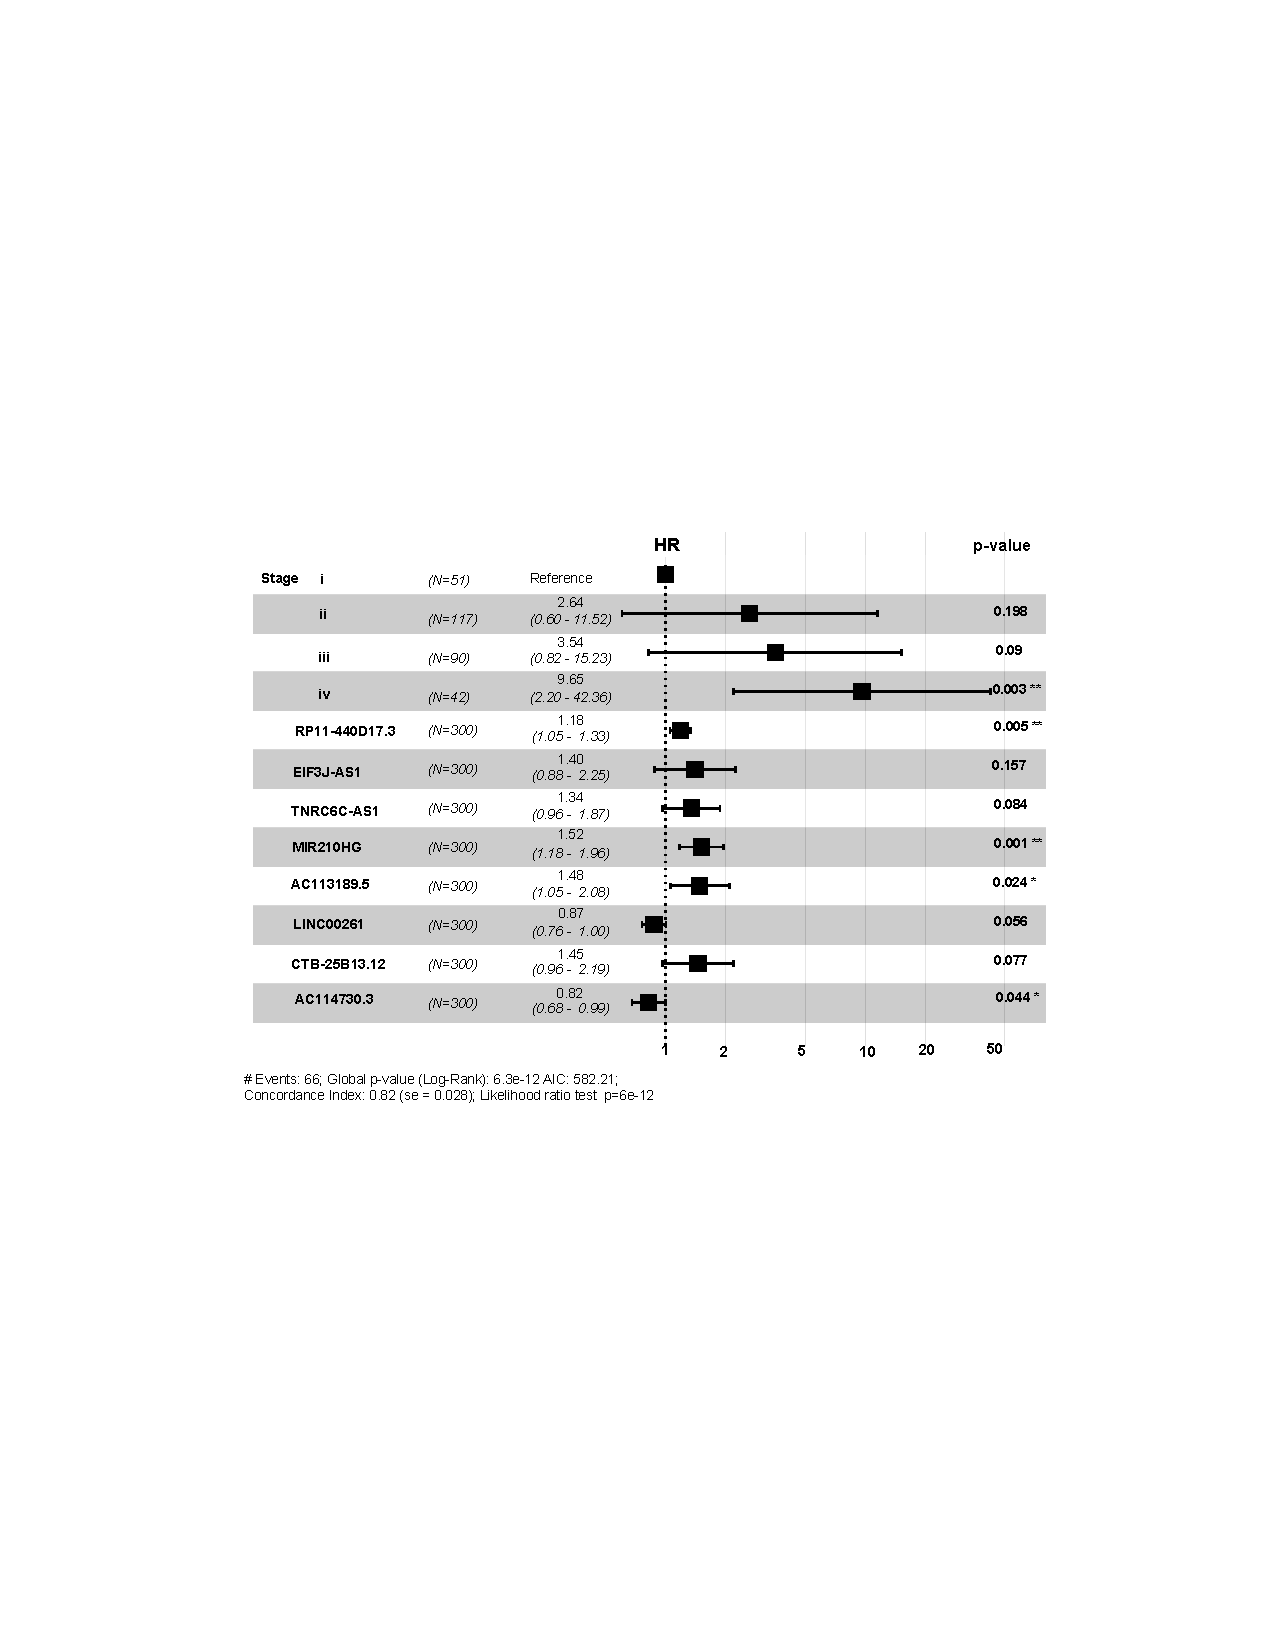
\includegraphics[width=\textwidth]{Figure-3}
\caption{Forest plot of the multivariate Cox proportional hazards model. Hazard ratios with 95\% confidence intervals and Wald test $p$-values for the eight lncRNAs and pathological stage.}
\label{fig3}
\end{figure}

\begin{figure}[htp]
\centering
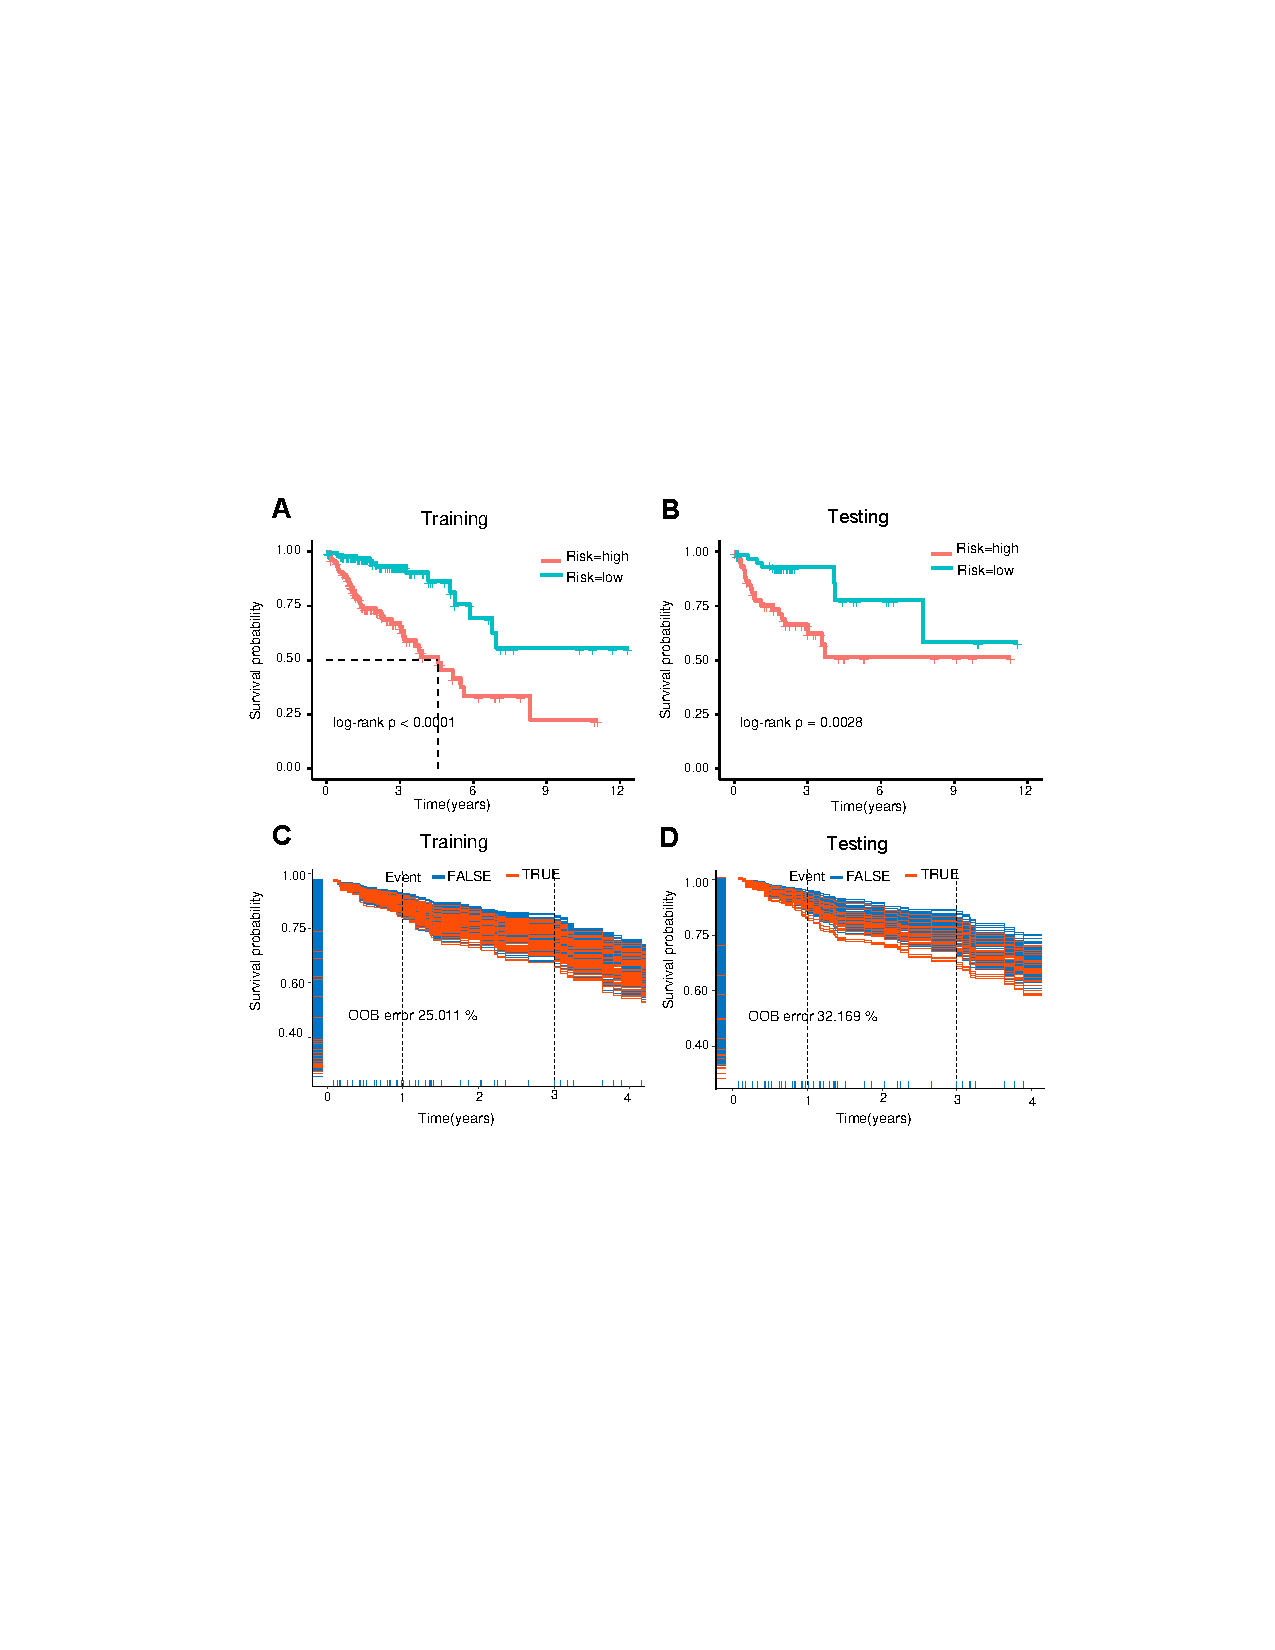
\includegraphics[width=\textwidth]{Figure-4}
\caption{Survival risk stratification. \textbf{(A,B)} Kaplan--Meier curves for high- and low-risk groups. \textbf{(C,D)} Random survival forest predicted survival with OOB error rates.}
\label{fig4}
\end{figure}

\begin{figure}[htp]
\centering
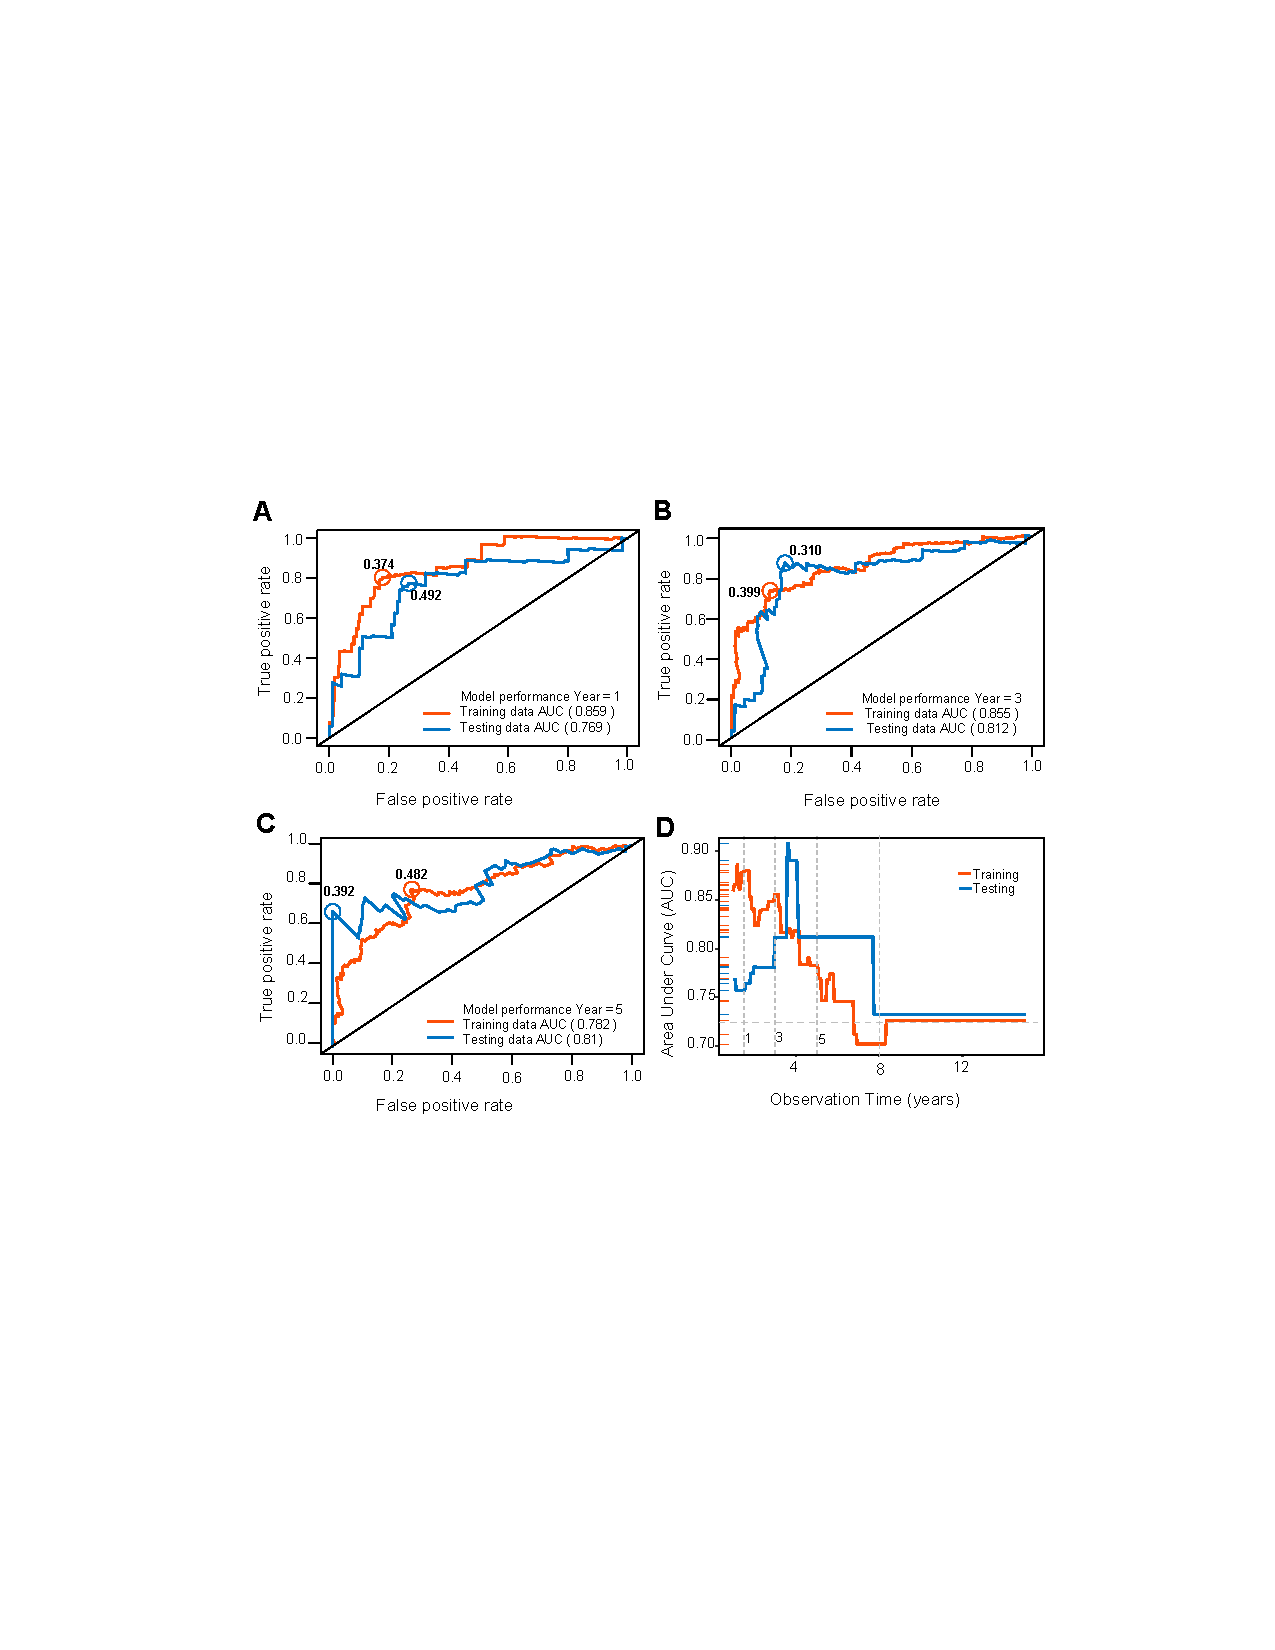
\includegraphics[width=\textwidth]{Figure-5}
\caption{Time-dependent ROC analysis of the relative risk score. \textbf{(A--C)} ROC curves at representative time points. \textbf{(D)} Trajectory of time-dependent AUC.}
\label{fig5}
\end{figure}

\begin{figure}[htp]
\centering
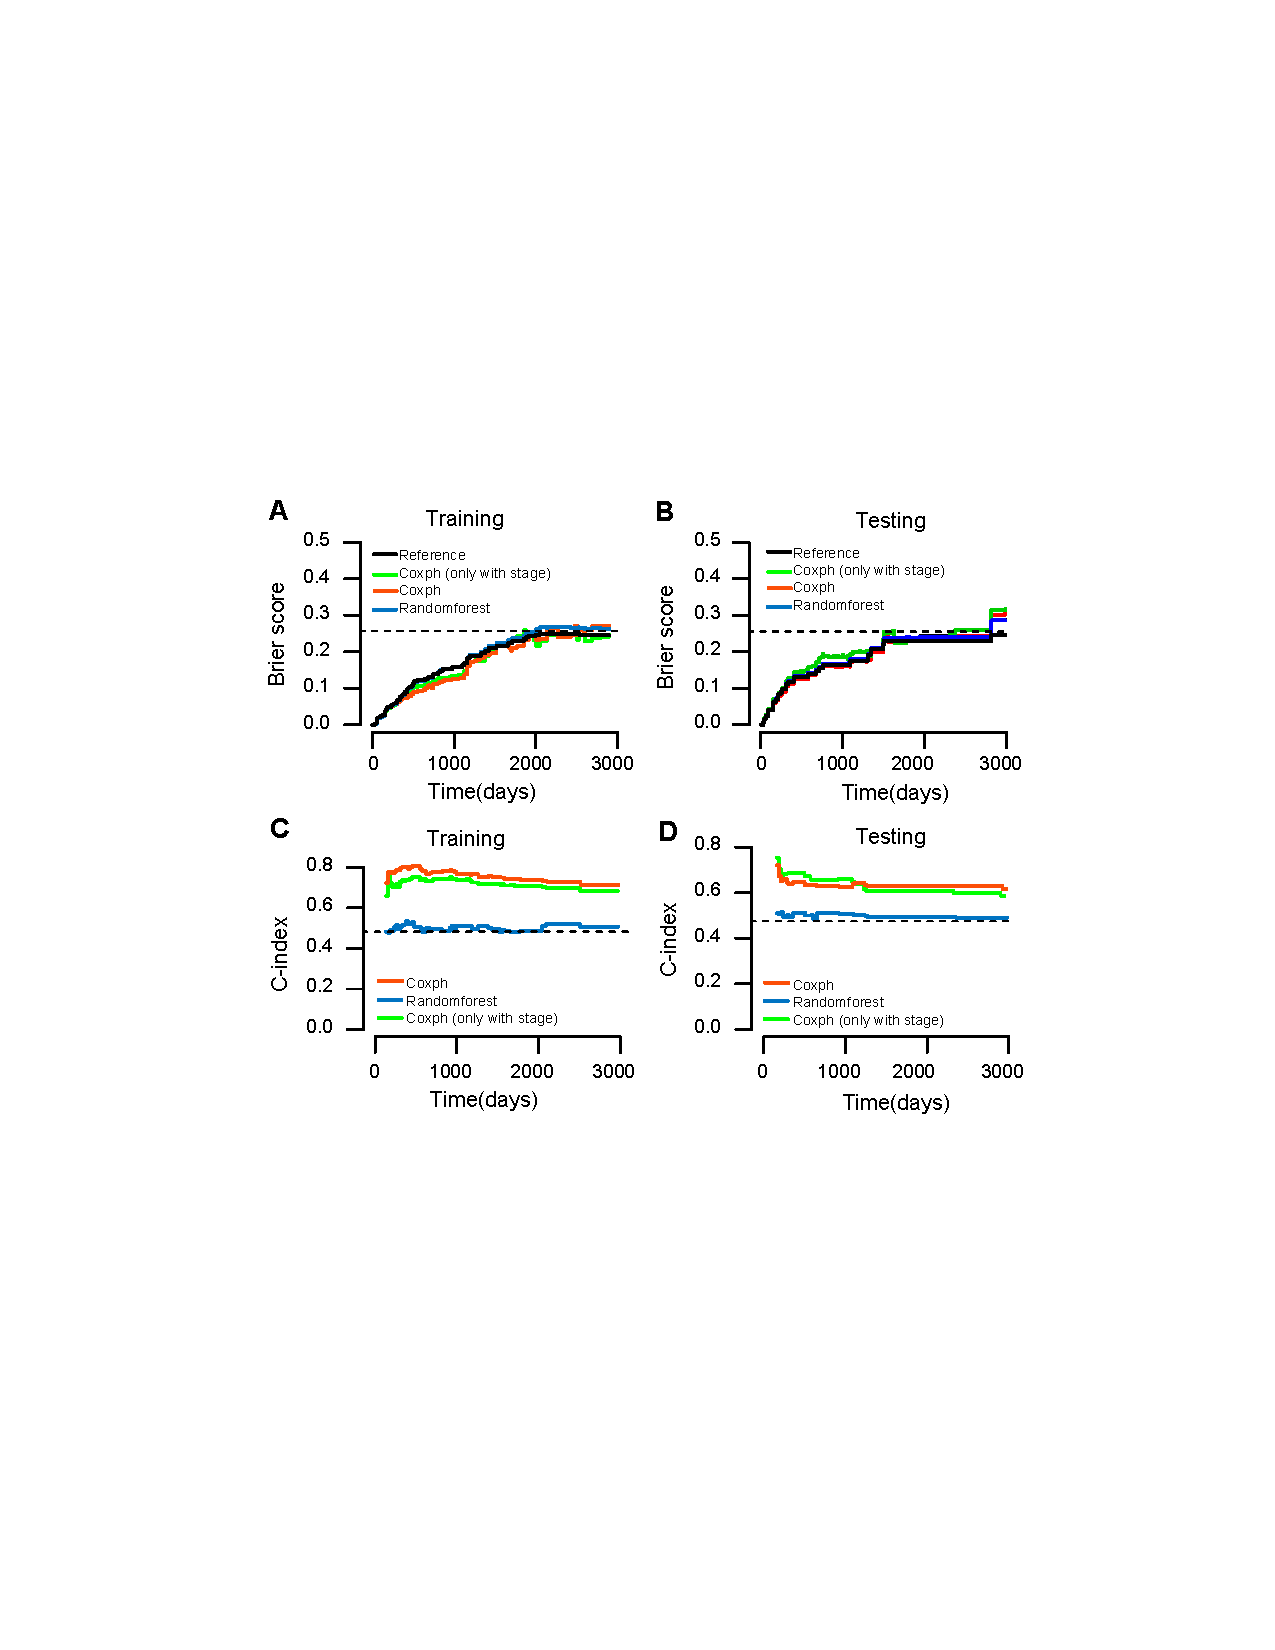
\includegraphics[width=\textwidth]{Figure-6}
\caption{Comparison of survival model performance. \textbf{(A,B)} Time-dependent Brier scores. \textbf{(C,D)} Concordance index over time.}
\label{fig6}
\end{figure}

\subsection{Diagnostic Classification Using lncRNA Expression Profiles}

To evaluate the diagnostic potential of the identified lncRNA panel, we constructed five binary classification models using the TCGA--GTEx expression data. These models distinguished tumor from non-tumor samples and included: logistic regression (baseline), elastic-net regularized logistic regression, support vector machine (SVM) with radial basis function kernel, random forest, and neural network. The data were split into training (70\%) and testing (30\%) sets with balanced class distributions. All models were trained with five repeats of tenfold cross-validation for hyperparameter optimization (Supplementary Figure~S2).

Classification performance metrics are summarized in Table~\ref{tab2}. Logistic regression and elastic-net logistic regression showed moderate performance (testing accuracy: 72.8\% and 73.3\%, respectively; AUC: 0.792 and 0.794). In contrast, the three strong classifiers achieved substantially higher accuracy in both training and testing sets: SVM (training: 97.8\%, testing: 91.6\%), random forest (training: 100\%, testing: 92.2\%), and neural network (training: 98.2\%, testing: 90.6\%). The corresponding AUC values were 0.974 (SVM), 0.980 (random forest), and 0.963 (neural network), demonstrating excellent discriminative ability (Figure~\ref{fig7}).

Cumulative gain lift curves confirmed these patterns: SVM, random forest, and neural network showed substantially enhanced response rates relative to a random classifier, capturing the majority of true positives within the top percentiles of predicted probability. The close agreement between training and testing performance for all models, particularly SVM and neural network, suggests that these classifiers generalize well and are not merely overfitting the training data.

\begin{table}[htp]
\centering
\caption{Performance of classification models on training and testing data.}
\small
\begin{tabular}{llcccccc}
\toprule
\textbf{Classifier} & \textbf{Set} & \textbf{Accuracy} & \textbf{AUC} & \textbf{Precision} & \textbf{Recall} & \textbf{F1} \\
\midrule
Logistic Reg. & Training & 0.679 & 0.792 & 0.648 & 0.636 & 0.642 \\
 & Testing & 0.728 & 0.792 & 0.701 & 0.701 & 0.701 \\
Elastic Net & Training & 0.674 & 0.793 & 0.642 & 0.636 & 0.639 \\
 & Testing & 0.733 & 0.794 & 0.700 & 0.724 & 0.712 \\
SVM & Training & 0.978 & 0.996 & 0.975 & 0.975 & 0.975 \\
 & Testing & 0.916 & 0.974 & 0.918 & 0.897 & 0.907 \\
Random Forest & Training & 1.000 & 1.000 & 1.000 & 1.000 & 1.000 \\
 & Testing & 0.922 & 0.980 & 0.919 & 0.908 & 0.913 \\
Neural Network & Training & 0.982 & 0.999 & 0.985 & 0.975 & 0.980 \\
 & Testing & 0.906 & 0.963 & 0.960 & 0.828 & 0.889 \\
\bottomrule
\end{tabular}
\label{tab2}
\end{table}

\begin{figure}[htp]
\centering
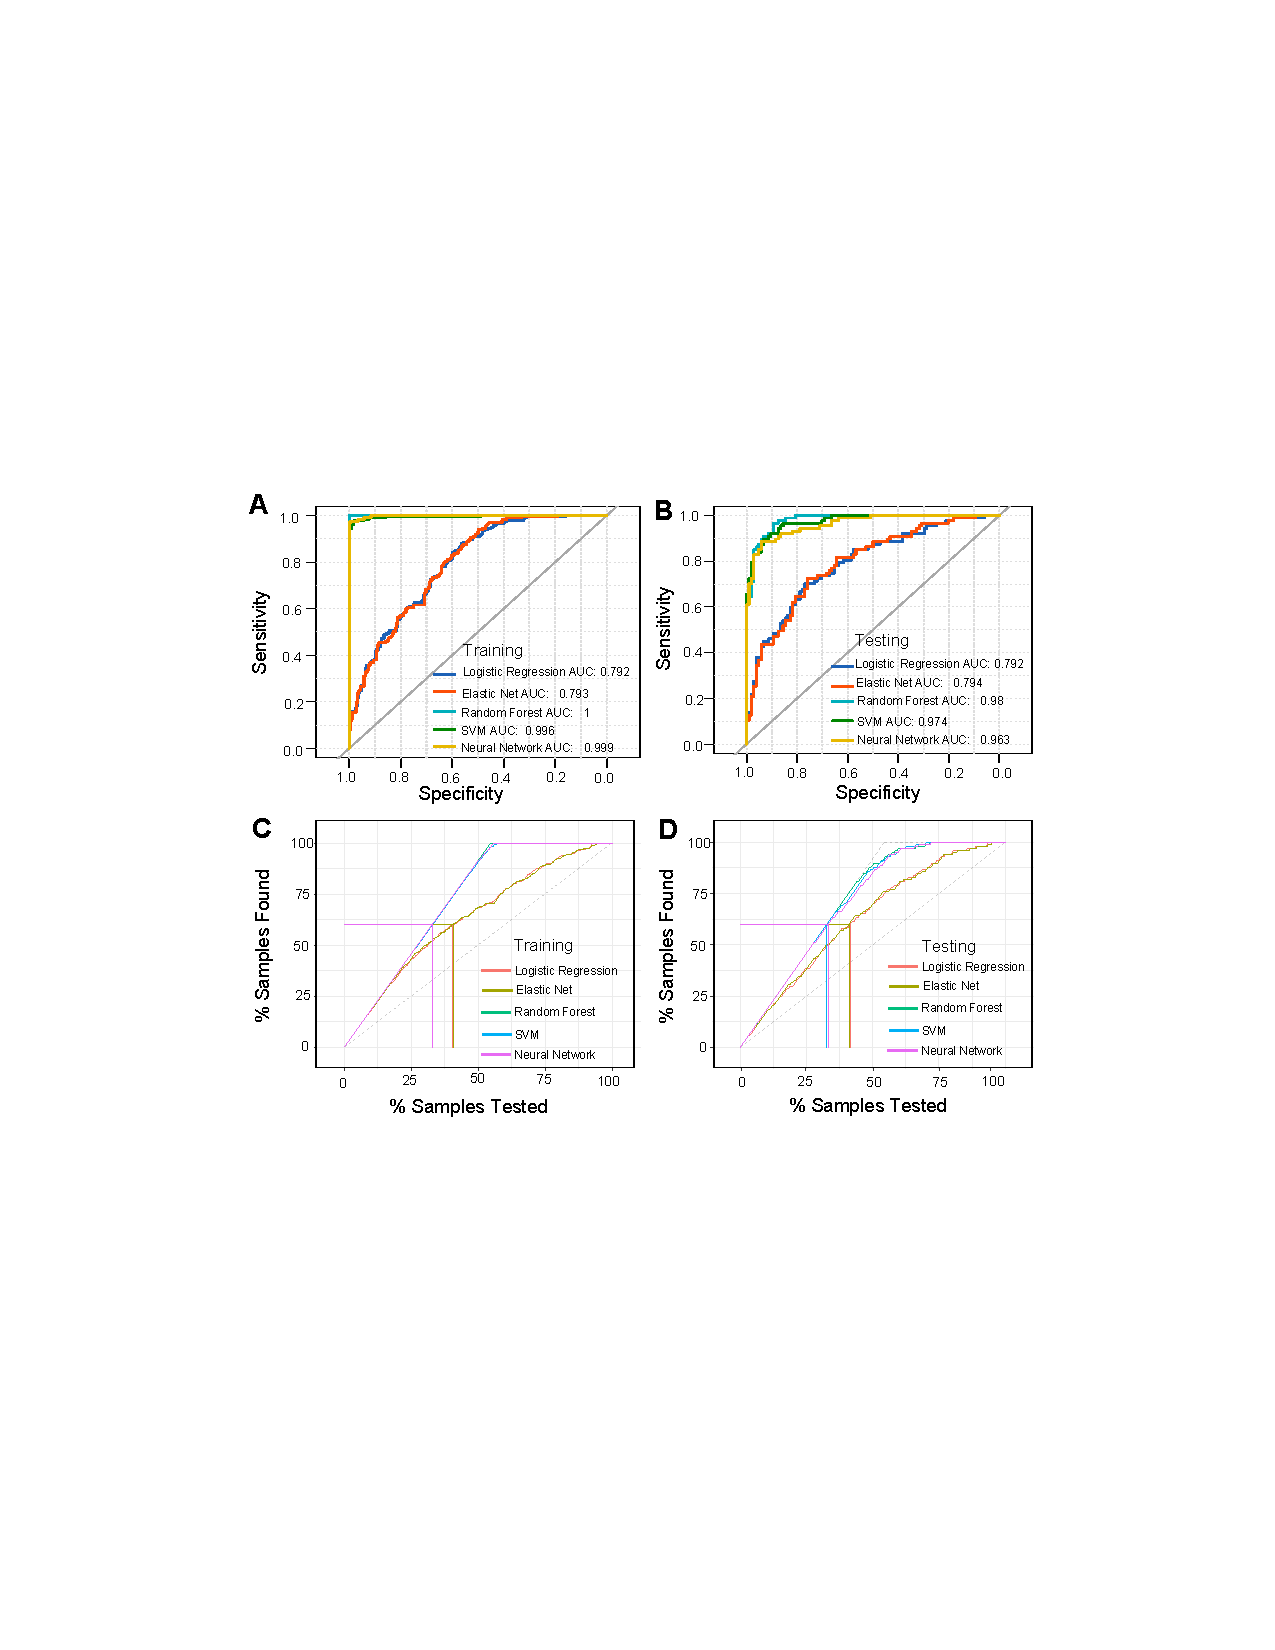
\includegraphics[width=\textwidth]{Figure-7}
\caption{ROC and lift curves for classification models. \textbf{(A,B)} ROC curves for all five classifiers. \textbf{(C,D)} Cumulative gain lift curves.}
\label{fig7}
\end{figure}

\section{Discussion}

In this study, we developed and validated a machine learning-based computational pipeline for discovering lncRNA signatures with dual diagnostic and prognostic utility in CRC. By integrating differential expression analysis with regularized Cox regression for feature selection, we identified an 8-lncRNA panel (RP11-440D17.3, EIF3J-AS1, TNRC6C-AS1, MIR210HG, AC113189.5, LINC00261, CTB-25B13.12, and AC114730.3) that, together with pathological stage, enabled robust patient risk stratification and accurate discrimination of tumor from normal samples.

Our prognostic model builds on the Cox proportional hazards framework, which remains the most widely used and interpretable approach for survival analysis in clinical research. The relative risk score stratified patients into groups with significantly different survival outcomes, with a time-dependent AUC that stabilized at 0.725 after 8 years. This performance is consistent with published lncRNA-based prognostic signatures for CRC: Qu et al.\ reported an 11-lncRNA signature with 3-year AUC of 0.801 for stage II colon cancer recurrence, while Xiong et al.\ described an 8-lncRNA RAS-related classifier with AUC of 0.717~\cite{ref16}. A succinylation-associated 6-lncRNA model achieved 5-year AUC of 0.802~\cite{ref17}. The higher AUCs reported in some studies (up to 0.920) typically incorporate additional clinical variables in nomogram frameworks and focus on shorter prediction horizons. Our model's strength lies in its parsimony---only eight features plus stage---and its stable long-term performance over 8 years of follow-up. The addition of lncRNA expression data consistently improved prediction performance over a model using pathological stage alone, reinforcing the clinical value of molecular signatures as complementary prognostic tools.

An important finding was that the random survival forest model, despite its theoretical flexibility in capturing non-linear relationships and complex interactions, underperformed relative to the Cox model on the testing data (OOB error: 32.169\% vs.\ 25.011\% on training data). This discrepancy likely reflects overfitting to the training set, a known challenge for tree-based ensemble methods when the number of features is small and the event rate is moderate. The RSF training-to-testing AUC drop observed here mirrors the pattern reported for RSF models in other CRC transcriptomic studies, where training AUCs of 0.927 collapsed to 0.618 on external validation. This raises important questions about the generalizability of complex survival models in modestly sized genomic datasets.

For the diagnostic classification task, SVM, random forest, and neural network all achieved testing accuracies exceeding 90\%, substantially outperforming both logistic regression variants. The strong agreement between training and testing performance indicates that overfitting was well controlled through repeated cross-validation. Notably, diagnostic classification performance is rarely evaluated in comparable lncRNA signature studies, which focus predominantly on prognostic modeling. Li et al.\ previously applied SVM to an 8-lncRNA classifier for CRC prognosis, while our study extends this to a systematic five-algorithm comparison with both diagnostic and prognostic endpoints. These results suggest that the 8-lncRNA expression signature contains sufficient information to reliably distinguish CRC from normal colon tissue, supporting its potential utility as a non-invasive molecular diagnostic tool.

Several of the identified lncRNAs have been independently implicated in cancer biology. Prior studies have reported EIF3J-AS1 as a regulator of multidrug resistance through autophagy induction in gastric cancer~\cite{ref28} and as a component of a recurrence-free survival signature in hepatocellular carcinoma~\cite{ref29}. MIR210HG has been extensively validated as an oncogenic lncRNA and prognostic biomarker in both colorectal adenocarcinoma and hepatocellular carcinoma~\cite{ref30,ref31}. Recent mechanistic studies have revealed that MIR210HG promotes colon cancer cell proliferation through multiple pathways: by binding PCBP1 to inhibit ferroptosis, by serving as a downstream effector of CREB3-mediated transcriptional activation, and by sponging miR-1226-3p as a competing endogenous RNA. Notably, a 2023 succinylation-associated lncRNA study independently selected MIR210HG in a 6-lncRNA prognostic signature for colon cancer, providing orthogonal validation. LINC00261 suppresses gastric cancer progression by promoting Slug degradation~\cite{ref32}. The fact that our purely data-driven feature selection procedure recovered lncRNAs with established biological relevance provides independent validation of the pipeline's ability to identify functionally meaningful candidates. Conversely, several lncRNAs in our panel remain largely uncharacterized. RP11-440D17.3, AC113189.5, and CTB-25B13.12 have no published functional studies to date, while AC114730.3 was recently included in an m6A-related 10-lncRNA prognostic signature for colon cancer but lacks direct mechanistic validation. TNRC6C-AS1 has appeared only in a pyroptosis-associated lncRNA signature without functional characterization. These poorly characterized lncRNAs represent potentially novel targets for experimental investigation and highlight the discovery potential of our data-driven pipeline.

This study has several limitations. First, the prognostic models were trained and tested on a single-institution dataset (TCGA-COAD) using random split validation; external validation on independent cohorts such as GSE39582 is essential to confirm generalizability. Second, clinical covariates had substantial missing data, limiting adjustment for known confounders beyond pathological stage. Third, the sample size, while among the larger studies of its kind, remains modest for machine learning applications. Fourth, the biological functions of several lncRNAs in our panel remain uncharacterized, requiring functional validation through \textit{in vitro} and \textit{in vivo} experiments. Finally, the clinical interpretability of non-linear classifiers (SVM, neural network) remains limited, which may pose challenges for translation into practice. Future work should prioritize external cohort validation, functional characterization of novel lncRNAs, and prospective evaluation of clinical utility.

\section{Ethics Statement}

This study analyzed publicly available, de-identified data from TCGA and GTEx. No human subjects were directly involved, and no new data were collected. All analyses were conducted in accordance with the data use policies of the respective repositories.

\section{Data Availability Statement}

All R scripts and documentation for reproducible analysis are publicly available at \url{https://github.com/woodhaha/CRC_data_mining}. The TCGA--GTEx harmonized expression data are available from the UCSC Xena platform (\url{https://toil.xenahubs.net}). TCGA-COAD data are available from the NCI Genomic Data Commons (\url{https://portal.gdc.cancer.gov}).

\section{Author Contributions}

ZZ, YB, and QX: conceptualization, methodology, software, formal analysis, writing---original draft. ZZ, ZX, and SH: supervision, writing---review and editing. All authors reviewed and approved the final manuscript.

\section{Funding}

This work was supported by the National Natural Science Foundation of China (No. 81272493, 81472213), the Health Commission of Zhejiang Province (No. 2019331258, No. 2019335600), and the Natural Sciences Foundation of Zhejiang Province (No. LY17H220001).

\section{Conflict of Interest}

The authors declare that the research was conducted in the absence of any commercial or financial relationships that could be construed as a potential conflict of interest.

\section{Supplementary Material}

The Supplementary Material for this article includes: baseline characteristics of the training and testing cohorts (Table~S1); distribution of lncRNA features and relative risk scores across patient groups (Table~S2); expression heatmaps and risk score distributions (Figure~S1); and hyperparameter tuning profiles for all five classification models (Figure~S2).

\begin{thebibliography}{99}
\raggedright

\bibitem{ref1} Sung H, Ferlay J, Siegel RL, et al. Global cancer statistics 2020: GLOBOCAN estimates of incidence and mortality worldwide for 36 cancers in 185 countries. \textit{CA Cancer J Clin}. 2021;71(3):209--249. doi:10.3322/caac.21660

\bibitem{ref2} Wang J, et al. Regulatory roles of long non-coding RNAs implicated in cancer hallmarks. \textit{Int J Cancer}. 2019. doi:10.1002/ijc.32277

\bibitem{ref3} Wang Q, et al. Long noncoding RNA LINC02023 regulates PTEN stability and suppresses tumorigenesis of colorectal cancer in a PTEN-dependent pathway. \textit{Cancer Lett}. 2019;451:68--78. doi:10.1016/j.canlet.2019.02.041

\bibitem{ref4} Wang YQ, et al. SATB2-AS1 suppresses colorectal carcinoma aggressiveness by inhibiting SATB2-dependent Snail transcription and epithelial-mesenchymal transition. \textit{Cancer Res}. 2019. doi:10.1158/0008-5472.CAN-18-2900

\bibitem{ref5} Yang C, et al. Long noncoding RNA HCP5 contributes to epithelial-mesenchymal transition in colorectal cancer through ZEB1 activation and interacting with miR-139-5p. \textit{Am J Transl Res}. 2019;11:953--963.

\bibitem{ref6} Kim T, Croce CM. Long noncoding RNAs: Undeciphered cellular codes encrypting keys of colorectal cancer pathogenesis. \textit{Cancer Lett}. 2018;417:89--95. doi:10.1016/j.canlet.2017.12.033

\bibitem{ref7} Batista PJ, Chang HY. Long noncoding RNAs: cellular address codes in development and disease. \textit{Cell}. 2013;152:1298--307. doi:10.1016/j.cell.2013.02.012

\bibitem{ref8} Wahlestedt C. Targeting long non-coding RNA to therapeutically upregulate gene expression. \textit{Nat Rev Drug Discov}. 2013;12:433--46. doi:10.1038/nrd4018

\bibitem{ref9} Cancer Genome Atlas Research Network, et al. The Cancer Genome Atlas Pan-Cancer analysis project. \textit{Nat Genet}. 2013;45:1113--20. doi:10.1038/ng.2764

\bibitem{ref10} GTEx Consortium. The Genotype-Tissue Expression (GTEx) pilot analysis: multitissue gene regulation in humans. \textit{Science}. 2015;348:648--60. doi:10.1126/science.1262110

\bibitem{ref11} Vivian J, et al. Toil enables reproducible, open source, big biomedical data analyses. \textit{Nat Biotechnol}. 2017;35:314--316. doi:10.1038/nbt.3772

\bibitem{ref12} Vidyasagar M. Identifying predictive features in drug response using machine learning: opportunities and challenges. \textit{Annu Rev Pharmacol Toxicol}. 2015;55:15--34. doi:10.1146/annurev-pharmtox-010814-124502

\bibitem{ref13} Kourou K, Exarchos TP, Exarchos KP, Karamouzis MV, Fotiadis DI. Machine learning applications in cancer prognosis and prediction. \textit{Comput Struct Biotechnol J}. 2015;13:8--17. doi:10.1016/j.csbj.2014.11.005

\bibitem{ref14} Wenric S, Shemirani R. Using supervised learning methods for gene selection in RNA-seq case-control studies. \textit{Front Genet}. 2018;9:297. doi:10.3389/fgene.2018.00297

\bibitem{ref15} Kuhn M. Building predictive models in R using the caret package. \textit{J Stat Softw}. 2008;28:1--26. doi:10.18637/jss.v028.i05

\bibitem{ref16} Zhang X, Wang J, Li J, Chen W, Liu C. CRlncRC: a machine learning-based method for cancer-related long noncoding RNA identification using integrated features. \textit{BMC Med Genomics}. 2018;11:120. doi:10.1186/s12920-018-0436-9

\bibitem{ref17} Chandra Gupta S, Nandan Tripathi Y. Potential of long non-coding RNAs in cancer patients: from biomarkers to therapeutic targets. \textit{Int J Cancer}. 2017;140:1955--1967. doi:10.1002/ijc.30546

\bibitem{ref18} Foster KR, Koprowski R, Skufca JD. Machine learning, medical diagnosis, and biomedical engineering research---commentary. \textit{Biomed Eng Online}. 2014;13:94. doi:10.1186/1475-925X-13-94

\bibitem{ref19} Deng M, Bragelmann J, Kryukov I, Saraiva-Agostinho N, Perner S. FirebrowseR: an R client to the Broad Institute's Firehose pipeline. \textit{Database (Oxford)}. 2017. doi:10.1093/database/baw160

\bibitem{ref20} Ritchie ME, et al. limma powers differential expression analyses for RNA-sequencing and microarray studies. \textit{Nucleic Acids Res}. 2015;43:e47. doi:10.1093/nar/gkv007

\bibitem{ref21} Sill M, Hielscher T, Becker N, Zucknick M. c060: Extended inference with lasso and elastic-net regularized Cox and generalized linear models. \textit{J Stat Softw}. 2014;62:1--22.

\bibitem{ref22} Bernau C, et al. Cross-study validation for the assessment of prediction algorithms. \textit{Bioinformatics}. 2014;30:i105--12. doi:10.1093/bioinformatics/btu279

\bibitem{ref23} Heagerty PJ, Lumley T, Pepe MS. Time-dependent ROC curves for censored survival data and a diagnostic marker. \textit{Biometrics}. 2000;56:337--44.

\bibitem{ref24} Chen HC, Kodell RL, Cheng KF, Chen JJ. Assessment of performance of survival prediction models for cancer prognosis. \textit{BMC Med Res Methodol}. 2012;12:102. doi:10.1186/1471-2288-12-102

\bibitem{ref25} Ishwaran H, Kogalur U, Blackstone E, Lauer M. Random survival forests. \textit{Ann Appl Stat}. 2008;2:841--860.

\bibitem{ref26} Mogensen UB, Ishwaran H, Gerds TA. Evaluating random forests for survival analysis using prediction error curves. \textit{J Stat Softw}. 2012;50:1--23.

\bibitem{ref27} Robin X, et al. pROC: an open-source package for R and S+ to analyze and compare ROC curves. \textit{BMC Bioinformatics}. 2011;12:77.

\bibitem{ref28} Luo Y, Zhou R, Huang N, Sun L, Liao W. Effect of long non-coding RNA EIF3J-AS1 on multi-drug resistance and autophagy in gastric cancer. \textit{J Clin Oncol}. 2017;35:e15581--e15581. doi:10.1200/JCO.2017.35.15\_suppl.e15581

\bibitem{ref29} Gu JX, et al. Six-long non-coding RNA signature predicts recurrence-free survival in hepatocellular carcinoma. \textit{World J Gastroenterol}. 2019;25:220--232. doi:10.3748/wjg.v25.i2.220

\bibitem{ref30} He Z, et al. Identification of LINC01234 and MIR210HG as novel prognostic signature for colorectal adenocarcinoma. \textit{J Cell Physiol}. 2019;234:6769--6777. doi:10.1002/jcp.27424

\bibitem{ref31} Wang Y, et al. MIR210HG predicts poor prognosis and functions as an oncogenic lncRNA in hepatocellular carcinoma. \textit{Biomed Pharmacother}. 2019;111:1297--1301. doi:10.1016/j.biopha.2018.12.134

\bibitem{ref32} Yu Y, et al. Long non-coding RNA LINC00261 suppresses gastric cancer progression via promoting Slug degradation. \textit{J Cell Mol Med}. 2017;21:955--967. doi:10.1111/jcmm.13035

\end{thebibliography}

\end{document}
